%%%%%%%%%%%%%%%%%%%%%%%%
% Sample use of the infthesis class to prepare an MSc thesis.
% This can be used as a template to produce your own thesis.
% Date: June 2019
%
%
% The first line specifies style options for taught MSc.
% You should add a final option specifying your degree.
% *Do not* change or add any other options.
%
% So, pick one of the following:
% \documentclass[msc,deptreport,adi]{infthesis}     % Adv Design Inf
% \documentclass[msc,deptreport,ai]{infthesis}      % AI
% \documentclass[msc,deptreport,cogsci]{infthesis}  % Cognitive Sci
% \documentclass[msc,deptreport,cs]{infthesis}      % Computer Sci
% \documentclass[msc,deptreport,cyber]{infthesis}   % Cyber Sec
% \documentclass[msc,deptreport,datasci]{infthesis} % Data Sci
% \documentclass[msc,deptreport,di]{infthesis}      % Design Inf
% \documentclass[msc,deptreport,inf]{infthesis}     % Informatics
%%%%%%%%%%%%%%%%%%%%%%%%

\documentclass[msc,deptreport.inf]{infthesis} % Do not change except to add your degree (see above).

% maths
\usepackage{amsmath}
\usepackage{amsfonts}
\usepackage{amssymb}
\newcommand{\matr}[1]{\mathbf{#1}}
\newcommand{\bgreek}[1]{\boldsymbol{#1}}
\newcommand{\R}{\mathbb R}
\newcommand{\E}{\mathbb E}
\newcommand{\N}{\mathbb N}
\newcommand{\diag}{\mathop{\mathrm{diag}}}

% algorithms
\usepackage{algorithm, algpseudocode}
\renewcommand{\algorithmicrequire}{\textbf{Input:}}
\renewcommand{\algorithmicensure}{\textbf{Output:}}

% graphics
\usepackage{graphicx}
\usepackage{subfig}


\begin{document}
\begin{preliminary}

\title{Extending the Bayesian Deep Learning Method MultiSWAG}

\author{Scott Brownlie}

\abstract{
  This skeleton demonstrates how to use the \texttt{infthesis} style
  for MSc dissertations in Artificial Intelligence, Cognitive Science,
  Computer Science, Data Science, and Informatics. It also emphasises
  the page limit, and that you must not deviate from the required
  style.  The file \texttt{skeleton.tex} generates this document and
  can be used as a starting point for your thesis. The abstract should
  summarise your report and fit in the space on the first page.
}

\maketitle

\section*{Acknowledgements}
Any acknowledgements go here.

\tableofcontents
\end{preliminary}


\chapter{Introduction}

%The preliminary material of your report should contain:
%\begin{itemize}
%\item
%The title page.
%\item
%An abstract page.
%\item
%Optionally an acknowledgements page.
%\item
%The table of contents.
%\end{itemize}
%
%As in this example \texttt{skeleton.tex}, the above material should be
%included between:
%\begin{verbatim}
%\begin{preliminary}
%    ...
%\end{preliminary}
%\end{verbatim}
%This style file uses roman numeral page numbers for the preliminary material.
%
%The main content of the dissertation, starting with the first chapter,
%starts with page~1. \emph{\textbf{The main content must not go beyond page~40.}}
%
%The report then contains a bibliography and any appendices, which may go beyond
%page~40. The appendices are only for any supporting material that's important to
%go on record. However, you cannot assume markers of dissertations will read them.
%
%You may not change the dissertation format (e.g., reduce the font
%size, change the margins, or reduce the line spacing from the default
%1.5 spacing). Over length or incorrectly-formatted dissertations will
%not be accepted and you would have to modify your dissertation and
%resubmit.  You cannot assume we will check your submission before the
%final deadline and if it requires resubmission after the deadline to
%conform to the page and style requirements you will be subject to the
%usual late penalties based on your final submission time.
%
%\section{Using Sections}
%
%Divide your chapters into sub-parts as appropriate.
%
%\section{Citations}
%
%Citations (such as \cite{P1} or \cite{P2}) can be generated using
%\texttt{BibTeX}. For more advanced usage, the \texttt{natbib} package is
%recommended. You could also consider the newer \texttt{biblatex} system.
%
%These examples use a numerical citation style. You may also use
%(Author, Date) format if you prefer.
%
%\chapter{Your next chapter}
%
%A dissertation usually contains several chapters.

\chapter{Factor Analysis}\label{sec:fa}

FA is a latent variable model which generates observations $\theta \in \R^d$ as follows. First, a latent vector $\matr{h} \in \R^K$, for some $K < d$, is sampled from $p(\matr{h}) = \mathcal{N}(\matr{0}, \matr{I})$. Next, $\matr{h}$ is transformed onto a $K$-dimensional linear subspace of $\R^d$ by left-multiplying it by a \emph{factor loading} matrix $\matr{F} \in \R^{d \times K}$. The origin of this subspace is then shifted by adding a bias term $\matr{c} \in \R^d$. Finally, the data is perturbed by adding some zero mean Gaussian noise $\epsilon \in \R^d$ sampled from $\mathcal{N}(\matr{0}, \Psi)$, where $\Psi$ is a $d\times d$ diagonal matrix \cite{barber2007}. Putting all this together, an observation $\theta \in \R^d$ is generated according to 
\begin{equation}\label{eqn:fa_model}
	\theta = \matr{Fh} + \matr{c} + \epsilon.
\end{equation}
In this context, an observation $\theta$ is the parameter vector of a neural network. 

It follows that, given $\matr{h}$, the observations $\theta$ are Gaussian distributed with mean $\matr{Fh} + \matr{c}$ and covariance $\Psi$ \cite{barber2007}. Formally,
\begin{equation}\label{eqn:fa_cond_dist}
	p(\theta | \matr{h}) 
	= \mathcal{N}\Big( \matr{Fh} + \matr{c}, \Psi \Big)
	= \frac{1}{\sqrt{(2\pi)^d |\Psi|}} 
	\exp \Big(-\frac{1}{2} (\theta - \matr{Fh} - \matr{c})^\intercal \Psi^{-1} (\theta - \matr{Fh} 	- \matr{c})\Big),
\end{equation}
where $|\Psi|$ is the \emph{determinant} of $\Psi$. From \cite{barber2007}, integrating $p(\theta | \matr{h})$ over $\matr{h}$ gives the marginal distribution
\begin{equation}\label{eqn:fa_marginal_dist}
	p(\theta) = \mathcal{N}\big(\matr{c}, \matr{FF}^{\intercal} + \Psi\big).
\end{equation}
The parameters of the model are $\matr{c}, \matr{F}$ and $\Psi$. The value of $\matr{c}$ which maximises the likelihood of the observed data is the empirical mean of the observations \cite{barber2007}, which in this case is $\theta_{\text{SWA}}$. 
%By substituting $\matr{c} = \theta_{\text{SWA}}$ into $p(\theta)$, the distribution in (\ref{eqn:fa_dist}) is obtained. 
Having set the bias term, an expectation maximisation (EM) or singular value decomposition (SVD) algorithm can find the maximum likelihood estimates of $\matr{F}$ and $\Psi$ \cite{barber2007}. However, both methods require storing all the observations in memory, making them impractical for high-dimensional data, such as the parameter vectors of deep neural networks. Two alternative online algorithms are presented in Sections \ref{sec:gradient_fa} and \ref{sec:online_em}.

\section{Online Stochastic Gradient Ascent}\label{sec:gradient_fa}

In situations where learning latent variable models with the classic EM algorithm is slow, \cite{barber2007} suggests optimising the log-likelihood of the model parameters via gradient methods. Since FA is a latent variable model, this approach can be applied here. 

In this case, the log-likelihood of the parameters $\matr{F}$ and $\Psi$ given the observed data, $\theta_1,\dots,\theta_T$, is 
\begin{equation}
	L(\matr{F}, \Psi) = \frac{1}{T} \sum_{t=1}^T \log p(\theta_t | \matr{F}, \Psi).
\end{equation}
The partial derivatives of the log-likelihood with respect to $\matr{F}$ and $\Psi$ are therefore
\begin{equation}
	\nabla_{\matr{F}, \Psi} L(\matr{F}, \Psi) = \frac{1}{T} \sum_{t=1}^T \nabla_{\matr{F}, \Psi} \log p(\theta_t | \matr{F}, \Psi).
\end{equation}
Computing $\nabla_{\matr{F}, \Psi} L(\matr{F}, \Psi)$ in full would require a pass over all observations, $\theta_1, \dots, \theta_T$. However, a stochastic gradient algorithm can be used instead, as long as the expectation of the sample derivatives is proportional to $\nabla_{\matr{F}, \Psi} L(\matr{F}, \Psi)$. By using $\nabla_{\matr{F}, \Psi} \log p(\theta_t | \matr{F}, \Psi)$, $t=1,\dots,T$, as the sample derivatives, this condition clearly holds. Hence, as long as the partial derivatives $\nabla_{\matr{F}, \Psi} \log p(\theta_t | \matr{F}, \Psi)$ can be computed efficiently, they can be used in conjunction with SGD or any of its variants to optimise $\matr{F}$ and $\Psi$ online. 
%After each $\theta_t$ is sampled and used to perform a gradient step, it can immediately be discarded. 

By adapting an argument for general latent variable models in \cite{barber2007} to FA, the required sample derivatives can be written as
\begin{align}\label{eqn:grad_log_likelihood}
\begin{split}
	\nabla_{\matr{F}, \Psi} \log p(\theta_t | \matr{F}, \Psi) 
	& = \frac{1}{p(\theta_t | \matr{F}, \Psi)} \nabla_{\matr{F}, \Psi} p(\theta_t | \matr{F}, \Psi) \\
	& = \frac{1}{p(\theta_t | \matr{F}, \Psi)} \nabla_{\matr{F}, \Psi} \int_{\matr{h}_t} p(\theta_t, \matr{h}_t | \matr{F}, \Psi) \\
	& = \frac{1}{p(\theta_t | \matr{F}, \Psi)} \int_{\matr{h}_t} \nabla_{\matr{F}, \Psi} p(\theta_t, \matr{h}_t | \matr{F}, \Psi) \\
	& = \frac{1}{p(\theta_t | \matr{F}, \Psi)} \int_{\matr{h}_t} p(\theta_t, \matr{h}_t | \matr{F}, \Psi) \nabla_{\matr{F}, \Psi} \log p(\theta_t, \matr{h}_t | \matr{F}, \Psi) \\
	& = \int_{\matr{h}_t} \frac{p(\theta_t, \matr{h}_t | \matr{F}, \Psi)}{p(\theta_t | \matr{F}, \Psi)} \nabla_{\matr{F}, \Psi} \log p(\theta_t, \matr{h}_t | \matr{F}, \Psi) \\
	& = \int_{\matr{h}_t} p(\matr{h}_t | \theta_t, \matr{F}, \Psi) \nabla_{\matr{F}, \Psi} \log p(\theta_t, \matr{h}_t | \matr{F}, \Psi) \\
	& = \E_{p(\matr{h}_t | \theta_t, \matr{F}, \Psi)} \big[ \nabla_{\matr{F}, \Psi} \log p(\theta_t, \matr{h}_t | \matr{F}, \Psi) \big].
\end{split}
\end{align}
This is as far as the derivation in \cite{barber2007} goes. However, given the form of the FA model, it is possible to manipulate the sample derivatives further. In particular, using the fact that $\matr{h}_t \sim \mathcal{N}(\matr{0}, \matr{I})$ is independent from $\matr{F}$ and $\Psi$,
\begin{align}\label{eqn:grad_log_complete_likelihood}
\begin{split}
	\nabla_{\matr{F}, \Psi} \log p(\theta_t, \matr{h}_t | \matr{F}, \Psi)
	& = \nabla_{\matr{F}, \Psi} \log \big(p(\theta_t | \matr{h}_t, \matr{F}, \Psi)p(\matr{h}_t | \matr{F}, \Psi)\big) \\
	& = \nabla_{\matr{F}, \Psi} \log \big(p(\theta_t | \matr{h}_t, \matr{F}, \Psi)p(\matr{h}_t)\big) \\
	& = \nabla_{\matr{F}, \Psi} \big( \log p(\theta_t | \matr{h}_t, \matr{F}, \Psi) + \log p(\matr{h}_t)\big) \\
	& = \nabla_{\matr{F}, \Psi} \log p(\theta_t | \matr{h}_t, \matr{F}, \Psi).
\end{split}
\end{align}
Substituting Equation (\ref{eqn:grad_log_complete_likelihood}) into Equation (\ref{eqn:grad_log_likelihood}),
\begin{equation}\label{eqn:simplified_grad_log_likelihood}
	\nabla_{\matr{F}, \Psi} \log p(\theta_t | \matr{F}, \Psi)
	= \E_{p(\matr{h}_t | \theta_t, \matr{F}, \Psi)} \big[ \nabla_{\matr{F}, \Psi} \log p(\theta_t | \matr{h}_t, \matr{F}, \Psi) \big].
\end{equation}
Note that $p(\theta_t | \matr{h}_t, \matr{F}, \Psi)$ is just the Gaussian distribution in Equation (\ref{eqn:fa_cond_dist}), given $\matr{F}$ and $\Psi$. Hence, substituting $\matr{c} = \theta_{\text{SWA}}$ into Equation (\ref{eqn:fa_cond_dist}) and applying the logarithm,
\begin{align}\label{eqn:log_fa_cond_dist}
\begin{split}
	\log p(\theta_t | \matr{h}_t, \matr{F}, \Psi)
	& = -\frac{1}{2} (\theta_t - \matr{Fh}_t - \theta_{\text{SWA}})^\intercal \Psi^{-1} (\theta_t - \matr{Fh}_t - \theta_{\text{SWA}}) - \frac{1}{2} \log |\Psi| - \frac{d}{2} \log 2\pi \\
	& = -\frac{1}{2} (\matr{d}_t - \matr{Fh}_t)^\intercal \Psi^{-1} (\matr{d}_t - \matr{Fh}_t) - \frac{1}{2} \log |\Psi| - \frac{d}{2} \log 2\pi,
\end{split}
\end{align}
where $\matr{d}_t = \theta_t - \theta_{\text{SWA}}$. This is convenient, since Equation (\ref{eqn:log_fa_cond_dist}) can be differentiated with respect to both $\matr{F}$ and $\Psi$. Of course, this requires access to $\theta_{\text{SWA}}$, which is not available during training. As a compromise - and following the approach of the SWAG covariance approximation - $\theta_{\text{SWA}}$ can be replaced by the running average of the neural network's parameter vectors.

\subsection{Partial derivatives with respect to $\matr{F}$}

From \cite{petersen2012}, for any symmetric matrix $\matr{W}$,
\begin{equation}
	\nabla_{\matr{A}} (\matr{x} - \matr{As})^\intercal \matr{W} (\matr{x} - \matr{As}) = -2 \matr{W} (\matr{x} - \matr{As}) \matr{s}^\intercal.
\end{equation}
Hence, differentiating Equation (\ref{eqn:log_fa_cond_dist}) with respect to $\matr{F}$ gives
\begin{equation}
	\nabla_{\matr{F}} \log p(\theta_t | \matr{h}_t, \matr{F}, \Psi)
	= \Psi^{-1} (\matr{d}_t - \matr{Fh}_t) \matr{h}_t^\intercal.
\end{equation}
It then follows from Equation (\ref{eqn:simplified_grad_log_likelihood}) that $\nabla_{\matr{F}} \log p(\theta_t | \matr{F}, \Psi)$ is the expected value of $\Psi^{-1} (\matr{d}_t - \matr{Fh}_t) \matr{h}_t^\intercal$ over the distribution $p(\matr{h}_t | \theta_t, \matr{F}, \Psi)$. Letting $\E[\cdot]$ denote $\E_{p(\matr{h}_t | \theta_t, \matr{F}, \Psi)}[\cdot]$ to simplify the notation, 
\begin{align}\label{eqn:expected_derivatives_wrt_F}
\begin{split}
	\nabla_{\matr{F}} \log p(\theta_t | \matr{F}, \Psi) 
	& = \E \big[ \Psi^{-1} (\matr{d}_t - \matr{Fh}_t) \matr{h}_t^\intercal \big] \\
	& = \Psi^{-1} \big(\E \big[ \matr{d}_t \matr{h}_t^\intercal \big] 
	- \E \big[ \matr{Fh}_t \matr{h}_t^\intercal \big] \big) \\
	& = \Psi^{-1}\big( \matr{d}_t \E \big[ \matr{h}_t^\intercal \big] 
	- \matr{F}  \E \big[ \matr{h}_t \matr{h}_t^\intercal \big]\big).
\end{split}
\end{align} 
From the E-step of the EM algorithm for FA in \cite{barber2007}, $p(\matr{h}_t | \theta_t, \matr{F}, \Psi) \propto \mathcal{N}(\matr{m}_t, \Sigma)$, where
\begin{equation}\label{eqn:variational_params}
	\Sigma = (\matr{I} + \matr{F}^\intercal \Psi^{-1} \matr{F})^{-1}
	\quad \text{and} \quad \matr{m}_t = \Sigma \matr{F}^\intercal \Psi^{-1} \matr{d}_t.
\end{equation}
Hence, using identities from \cite{petersen2012}, 
\begin{equation}\label{eqn:expected_value_h_hh}
	\E \big[ \matr{h}_t^\intercal \big] = \matr{m}_t^\intercal \quad \text{and} \quad \E \big[ \matr{h}_t \matr{h}_t^\intercal \big] = \Sigma + \matr{m}_t \matr{m}_t^\intercal.
\end{equation}
Finally, substituting Equation (\ref{eqn:expected_value_h_hh}) into Equation (\ref{eqn:expected_derivatives_wrt_F}), 
\begin{align}\label{eqn:derivatives_wrt_F}
\begin{split}
	\nabla_{\matr{F}} \log p(\theta_t | \matr{F}, \Psi) 
	& = \Psi^{-1} \big(\matr{d}_t \matr{m}_t^\intercal - \matr{F}  (\Sigma + \matr{m}_t \matr{m}_t^\intercal)\big).
\end{split}
\end{align} 

\subsection{Partial derivatives with respect to $\Psi$}

In order to differentiate Equation (\ref{eqn:log_fa_cond_dist}) with respect to $\Psi$, it helps to use the fact that $\Psi$ is diagonal. First consider $\matr{X}^{-1} = \diag(\frac{1}{x_1}, \dots, \frac{1}{x_d})$ and $\matr{a} = (a_1, \dots, a_d)^\intercal$. Then 
\begin{equation}\label{eqn:aXa}
	\matr{a}^\intercal \matr{X}^{-1} \matr{a} = \sum_{i=1}^d \frac{a_i^2}{x_i},
\end{equation}
and so
\begin{equation}
	\frac{\partial}{\partial x_i} \matr{a}^\intercal \matr{X}^{-1} \matr{a} = \frac{-a_i^2}{x_i^2}
\end{equation}
for $i=1, \dots, d$. Since the partial derivatives of Equation (\ref{eqn:aXa}) with respect to the off-diagonal entries of $\matr{X}$ are zero, 
\begin{align}\label{eqn:derivatives_diag_qaud_form}
\begin{split}
	\nabla_\matr{X} (\matr{a}^\intercal \matr{X}^{-1} \matr{a}) 
	& = \diag\Big({\frac{-a_1^2}{x_1^2}, \dots, \frac{-a_d^2}{x_d^2}}\Big) \\
	& = -\diag\big(\diag(\matr{X}^{-2}) \odot \matr{a}^2\big),
\end{split}
\end{align}  
where $\odot$ denotes the element-wise matrix product (with broadcasting, if applicable) and the square of a vector is applied element-wise. Also, when applied to a $d$-length vector, $\diag(\cdot)$ represents the $d \times d$ diagonal matrix with the vector on its diagonal, and when applied to a $d \times d$ matrix, $\diag(\cdot)$ represents the $d$-length vector consisting of the diagonal entries of the matrix. Substituting $\matr{X} = \Psi$ and $\matr{a} = \matr{d}_t - \matr{Fh}_t$, into Equation (\ref{eqn:derivatives_diag_qaud_form}),
\begin{equation}\label{eqn:derivatives_wrt_Psi_1}
	\nabla_\Psi (\matr{d}_t - \matr{Fh}_t)^\intercal \Psi^{-1} (\matr{d}_t - \matr{Fh}_t) 
	= -\diag\big(\diag(\Psi^{-2}) \odot (\matr{d}_t - \matr{Fh}_t)^2\big).
\end{equation}
Also, using the identity $\nabla_\matr{X} \log |\matr{X}| = \matr{X}^{-\intercal}$ from \cite{petersen2012} and the fact that $\Psi^{-\intercal} = \Psi^{-1}$, 
\begin{equation}\label{eqn:derivatives_wrt_Psi_2}
	\nabla_\Psi \log |\Psi|
	= \Psi^{-1}.
\end{equation}
Hence, the partial derivatives of Equation (\ref{eqn:log_fa_cond_dist}) with respect to $\Psi$ are
\begin{equation}
	\nabla_{\Psi} \log p(\theta_t | \matr{h}_t, \matr{F}, \Psi)
	= \frac{1}{2} \diag\big(\diag(\Psi^{-2}) \odot (\matr{d}_t - \matr{Fh}_t)^2\big) - \frac{1}{2}\Psi^{-1}.
\end{equation}
Again, letting $\E[\cdot]$ denote $\E_{p(\matr{h}_t | \theta_t, \matr{F}, \Psi)}[\cdot]$, it follows from Equation (\ref{eqn:simplified_grad_log_likelihood}) that
\begin{align}\label{eqn:expected_gradient}
\begin{split}
	2 \cdot \nabla_{\Psi} \log p(\theta_t | \matr{F}, \Psi) 
	& = \E \big[ \diag\big(\diag(\Psi^{-2}) \odot (\matr{d}_t - \matr{Fh}_t)^2\big) - \Psi^{-1} \big] \\
	& = \diag\Big(\E \big[\diag(\Psi^{-2}) \odot (\matr{d}_t - \matr{Fh}_t)^2\big]\Big) - \E \big[ \Psi^{-1} \big] \\
	& = \diag\Big(\diag(\Psi^{-2}) \odot \E \big[(\matr{d}_t - \matr{Fh}_t)^2\big]\Big) - \Psi^{-1}.
\end{split}
\end{align} 
Now, expanding the expectation inside Equation (\ref{eqn:expected_gradient}) and substituting in the expressions from Equation (\ref{eqn:expected_value_h_hh}),
\begin{align}\label{eqn:expected_gradient_d_Fh}
\begin{split}
	\E \big[(\matr{d}_t - \matr{Fh}_t)^2\big] 
	& = \E \big[\matr{d}_t \odot \matr{d}_t \big] - 2\E \big[ \matr{d}_t \odot (\matr{Fh}_t) \big] + \E \big[ (\matr{Fh}_t) \odot (\matr{Fh}_t) \big] \\
	& = \matr{d}_t \odot \matr{d}_t - 2\matr{d}_t \odot \big(\matr{F} \E \big[ \matr{h}_t \big]\big) + \E \big[ \diag(\matr{F}\matr{h}_t \matr{h}_t^\intercal  \matr{F}^\intercal) \big] \\
	& = \matr{d}_t \odot \matr{d}_t - 2\matr{d}_t \odot (\matr{F} \matr{m}_t) + \diag\big(\E \big[ \matr{F}\matr{h}_t \matr{h}_t^\intercal  \matr{F}^\intercal \big]\big) \\
	& = \matr{d}_t \odot \matr{d}_t - 2\matr{d}_t \odot (\matr{F} \matr{m}_t) + \diag\big( \matr{F} \E \big[ \matr{h}_t \matr{h}_t^\intercal \big] \matr{F}^\intercal \big) \\
	& = \matr{d}_t \odot \matr{d}_t - 2\matr{d}_t \odot (\matr{F} \matr{m}_t) + \diag\big( \matr{F} (\Sigma + \matr{m}_t \matr{m}_t^\intercal) \matr{F}^\intercal \big).
\end{split}
\end{align} 
Finally, substituting Equation (\ref{eqn:expected_gradient_d_Fh}) into Equation (\ref{eqn:expected_gradient}) and rearranging, 
\begin{align}
\begin{split}\label{eqn:derivatives_wrt_Psi}
	\nabla_{\Psi} \log p(\theta_t | \matr{F}, \Psi) 
	& = \diag\Bigg(\frac{1}{2} \diag(\Psi^{-2}) \odot \Big(\matr{d}_t \odot \matr{d}_t - 2\matr{d}_t \odot (\matr{F} \matr{m}_t) \\
	& \quad + \diag\big( \matr{F} (\Sigma + \matr{m}_t \matr{m}_t^\intercal) \matr{F}^\intercal \big) \Big) \Bigg)
	 - \frac{1}{2} \Psi^{-1}.
\end{split}
\end{align} 

\subsection{Practical implementation}

In practice, storing the full $d\times d$ covariance matrix $\Psi$ (or its inverse) would be infeasible for high-dimensional $\theta_t \in \R^d$. However, since $\Psi$ is diagonal and the partial derivatives of the log-likelihood with respect to the off-diagonal are always zero, it suffices to work with the diagonal entries only. All occurrences of $d \times d$ matrices can then be removed from the gradient calculations. 

First, note that the partial derivatives with respect to both $\matr{F}$ and $\Psi$ depend on $\matr{m}_t$ and $\Sigma$ from Equation (\ref{eqn:variational_params}), which themselves depend on  $\Psi^{-1}$. Let $\psi = \diag(\Psi)$ and $\psi^{-n} = \diag(\Psi^{-n})$ for $n \in \N^+$. Then 
\begin{equation}
	\matr{F}^\intercal \Psi^{-1} = (\matr{F} \odot \psi^{-1})^\intercal.
\end{equation}
Now, setting $\matr{C} =  (\matr{F} \odot \psi^{-1})^\intercal$ and substituting into Equation (\ref{eqn:variational_params}), it follows that 
\begin{equation}\label{eqn:efficient_m_and_sigma}
	\Sigma = (\matr{I} + \matr{C} \matr{F})^{-1} \quad \text{and} \quad \matr{m}_t = \Sigma \matr{C} \matr{d}_t.
\end{equation}
These more efficient values can then be used in Equation (\ref{eqn:derivatives_wrt_F}), which itself can be simplified to 
\begin{align}\label{eqn:efficient_derivatives_wrt_F}
\begin{split}
	\nabla_{\matr{F}} \log p(\theta_t | \matr{F}, \Psi) 
	& = \psi^{-1} \odot \big(\matr{d}_t \matr{m}_t^\intercal  - \matr{F}  (\Sigma + \matr{m}_t \matr{m}_t^\intercal) \big).
\end{split}
\end{align} 
Also, the partial derivatives with respect to $\Psi$ in Equation (\ref{eqn:derivatives_wrt_Psi}) can be re-written with respect to $\psi$, as 
\begin{align}
\begin{split}\label{eqn:efficient_derivatives_wrt_Psi}
	\nabla_{\psi} \log p(\theta_t | \matr{F}, \Psi) 
	& = \frac{1}{2} \psi^{-2} \odot \Big(\matr{d}_t \odot \matr{d}_t - 2\matr{d}_t \odot (\matr{F} \matr{m}_t) \\
	& \quad + \text{sum}\big((\matr{F} (\Sigma + \matr{m}_t \matr{m}_t^\intercal)) \odot \matr{F}, \text{ dim} = 1\big) \Big)
	 - \frac{1}{2} \psi^{-1},
\end{split}
\end{align} 
where $\text{sum}(\cdot, \text{ dim} = 1)$ denotes the operation of summing along the rows of a matrix. 

One final point is that the elements of $\psi$ must be positive, since they represent variances. One way to achieve this is by using the re-parameterisation $\psi = \exp \beta$ for some unconstrained parameter $\beta \in \R^d$. Then the gradient updates can be performed on $\beta$ instead of $\psi$. Using the chain rule from calculus, 
\begin{align}
\begin{split}\label{eqn:efficient_derivatives_wrt_beta}
	\nabla_{\beta} \log p(\theta_t | \matr{F}, \Psi)
	& = \nabla_{\psi} \log p(\theta_t | \matr{F}, \Psi) \odot \nabla_{\beta} \exp \beta \\
	& = \nabla_{\psi} \log p(\theta_t | \matr{F}, \Psi) \odot \exp \beta \\
	& = \nabla_{\psi} \log p(\theta_t | \matr{F}, \Psi) \odot \psi,
\end{split}
\end{align} 
where $\nabla_{\psi} \log p(\theta_t | \matr{F}, \Psi)$ is given in Equation (\ref{eqn:efficient_derivatives_wrt_Psi}).

Pseudo code for online stochastic gradient FA is given in Algorithm \ref{alg:gradient_fa}.

\begin{algorithm}[!htbp] 
	\caption{Online Stochastic Gradient Factor Analysis}
	\label{alg:gradient_fa}
	\begin{algorithmic}[1]
		\Require{Observation dimension $d$, latent dimension $K$, learning rate $\alpha > 0$} 
		\State Initialise $\matr{F} \in \R^{d \times K}$, $\psi > \matr{0} \in \R^d$, $\overline{\theta}_0 = \matr{0}^d$
		\State $\beta \leftarrow \log \psi$
		\For {$t=1,\dots,T$}
			\State Sample observation $\theta_t \in \R^d$
			\State
				$\overline{\theta}_t \leftarrow  \overline{\theta}_{t-1} + \frac{1}{t}\big(\overline{\theta}_t - \overline{\theta}_{t-1}\big)$
			\State $\matr{d}_t \leftarrow \theta_t - \overline{\theta}_t$
			\State $\matr{C} \leftarrow (\matr{F} \odot \psi^{-1})^\intercal$ (with broadcasting)
			\State $\Sigma \leftarrow (\matr{I} + \matr{C} \matr{F})^{-1}$ 
			\State $\matr{m}_t \leftarrow \Sigma \matr{C} \matr{d}_t$ 
			\State Compute $\nabla_{\matr{F}} \log p(\theta_t | \matr{F}, \Psi)$ 
			according to Equation (\ref{eqn:efficient_derivatives_wrt_F})
			\State Compute $\nabla_{\beta} \log p(\theta_t | \matr{F}, \Psi)$ 
			according to Equation (\ref{eqn:efficient_derivatives_wrt_beta})
			\State $\matr{F} \leftarrow \matr{F} + \alpha \nabla_{\matr{F}} \log p(\theta_t | \matr{F}, \Psi)$
			\State $\beta \leftarrow \beta + \alpha \nabla_{\beta} \log p(\theta_t | \matr{F}, \Psi)$
			\State $\psi \leftarrow \exp \beta$
		\EndFor
		\State $\theta_{\text{SWA}} \leftarrow \overline{\theta}_T$
		\State \Return $\theta_{\text{SWA}}, \matr{F}, \psi$
	\end{algorithmic}
\end{algorithm}


\section{Online EM}\label{sec:online_em}

The classic EM algorithm for FA iteratively optimises the log-likelihood of $\matr{F}$ and $\Psi$ by alternating ``E'' and ``M'' steps until convergence. Using properties of the Kullback-Leibler divergence, it can be shown that 
\begin{equation}\label{eqn:EM_bound}
	L(\matr{F}, \Psi) \geq 
	- \sum_{t=1}^T \E_{q(\matr{h}_t | \theta_t)} \big[\log q(\matr{h}_t | \theta_t)\big]
	+ \sum_{t=1}^T \E_{q(\matr{h}_t | \theta_t)} \big[\log p(\matr{h}_t, \theta_t | \matr{F}, \Psi)\big],
\end{equation}
where the first and second terms on the right-hand side are called the \emph{entropy} and \emph{energy}, respectively, and $q(\matr{h}_t | \theta_t)$, $t=1,\dots,T$, are known as the \emph{variational} distributions \cite{barber2007}. The EM algorithm optimises this lower bound on the log-likelihood with respect to $\matr{F}$, $\Psi$ and also $q(\matr{h}_t | \theta_t)$, hence the name ``variational distributions''. The idea is that, by pushing up the lower bound, the log-likelihood $L(\matr{F}, \Psi)$ will hopefully increase as well. In fact, it is guaranteed that each iteration of EM does not decrease $L(\matr{F}, \Psi)$, which again follows from the properties of the Kullback-Leibler divergence \cite{barber2007}.

\subsection{E-step}

In the batch E-step, $\matr{F}$ and $\Psi$ are fixed and Equation (\ref{eqn:EM_bound}) is maximised with respect to $q(\matr{h}_t | \theta_t)$, $t=1,\dots,T$. From \cite{barber2007}, the optimal variational distributions are 
\begin{equation}
	q(\matr{h}_t | \theta_t) = p(\matr{h}_t | \theta_t, \matr{F}, \Psi)  \propto \mathcal{N}(\matr{m}_t, \Sigma), 
\end{equation}
where $\matr{m}_t$ and $\Sigma$ are given in Equation (\ref{eqn:efficient_m_and_sigma}). Note that this optimisation can be performed separately for each $\theta_t$ as it is sampled, using the estimates of $\matr{F}$ and $\Psi$ on iteration $t$. However, in batch EM all $q(\matr{h}_t | \theta_t)$ are updated on every iteration. This is clearly not possible in an online algorithm which discards $\theta_t$ before sampling $\theta_{t + 1}$. Therefore, as a compromise, in the online version each $q(\matr{h}_t | \theta_t)$ will be computed once only, on iteration $t$, and held fixed thereafter. The only other detail is that the batch algorithm uses $\theta_{\text{SWA}}$ to compute $\matr{m}_t$. As $\theta_{\text{SWA}}$ is not available during training, it will be replaced by the running average of the neural network's parameter vectors, as in the online gradient-based FA algorithm from Section \ref{sec:gradient_fa}.


\subsection{M-step}

In the batch M-step, $q(\matr{h}_t | \theta_t)$, $t=1,\dots,T$, are fixed and Equation (\ref{eqn:EM_bound}) is maximised with respect to $\matr{F}$ and $\Psi$. From \cite{barber2007}, the optimal values are 
\begin{equation}
	\matr{F} = \matr{A}\matr{H}^{-1},
\end{equation}
where
\begin{equation}\label{eqn:em_A_and_H_update}
	\matr{A} = \frac{1}{T} \sum_{t=1}^T \matr{d}_t \matr{m}_t^\intercal \quad \text{and} \quad 
	\matr{H} = \Sigma + \frac{1}{T} \sum_{t=1}^T \matr{m}_t \matr{m}_t^\intercal,
\end{equation}
and
\begin{equation}\label{eqn:em_Psi_update}
	\Psi = \text{diag}\Bigg(\text{diag}\Bigg( \frac{1}{T} \sum_{t=1}^T \matr{d}_t \matr{d}_t^\intercal - 2\matr{FA}^\intercal + \matr{FHF}^\intercal \Bigg)\Bigg).
\end{equation}
Note that this optimisation involves summing over $t=1,\dots,T$. Moreover, on each iteration all components of the sums in Equation (\ref{eqn:em_A_and_H_update}) and Equation (\ref{eqn:em_Psi_update}) are updated. As in the E-step, updating all components is not possible in an online algorithm. Therefore, in the online version these sums will be updated incrementally on each iteration. 

\subsection{Practical implementation}

Let $\overline{\matr{A}}_t$ and $\overline{\matr{H}}_t$ be the estimates of $\matr{A}$ and $\matr{H}$ from Equation (\ref{eqn:em_A_and_H_update}), respectively, after iteration $t$ of online EM. That is,
\begin{equation}\label{eqn:em_A_and_H_incremental_update}
	\overline{\matr{A}}_t = \frac{1}{t} \sum_{i=1}^t \matr{d}_i \matr{m}_i^\intercal \quad \text{and} \quad 
	\overline{\matr{H}}_t = \Sigma + \frac{1}{t} \sum_{i=1}^t \matr{m}_i \matr{m}_i^\intercal.
\end{equation}
Then the estimates of $\matr{F}$ and $\Psi$ on iteration $t$ become
\begin{equation}
	\matr{F} = \overline{\matr{A}}_t \overline{\matr{H}}_t^{-1}
\end{equation}
and
\begin{equation}\label{eqn:em_Psi_incremental_update}
	\Psi = \text{diag}\Bigg(\text{diag}\Bigg( \frac{1}{t} \sum_{i=1}^t \matr{d}_i \matr{d}_i^\intercal - 2 \matr{F}\overline{\matr{A}}_t^\intercal + \matr{F}\overline{\matr{H}}_t \matr{F}^\intercal \Bigg)\Bigg).
\end{equation}
As in the online gradient-based FA algorithm from Section \ref{sec:gradient_fa}, it suffices to work with $\psi = \diag(\Psi)$ instead of $\Psi$. 
The diagonal entries of Equation (\ref{eqn:em_Psi_incremental_update}) can be computed more efficiently as 
\begin{align}
\begin{split}\label{eqn:em_Psi_efficient_update}
	\psi 
	& = \frac{1}{t} \sum_{i=1}^t \matr{d}_i^2 
	- 2 \cdot \text{sum} \big(\matr{F} \odot \overline{\matr{A}}_t, \text{ dim} = 1\big)
	+ \text{sum}\big((\matr{F} \overline{\matr{H}}_t) \odot \matr{F}, \text{ dim} = 1\big) \\	
	& = \frac{1}{t} \sum_{i=1}^t \matr{d}_i^2 
	+ \text{sum} \big((\matr{F} \overline{\matr{H}}_t) \odot \matr{F} -2\matr{F} \odot \overline{\matr{A}}_t , \text{ dim} = 1\big).
\end{split}
\end{align}
(TODO: check whether this can be negative).
All that remains to complete the online algorithm is to define the incremental update rules for $\overline{\matr{A}}_t$ and $\overline{\matr{H}}_t$. Both are similar, and for $\overline{\matr{A}}_t$ the derivation is 
\begin{align}
\begin{split}
	\overline{\matr{A}}_t 
	& = \frac{1}{t} \sum_{i=1}^t \matr{d}_i \matr{m}_i^\intercal \\
	& = \frac{1}{t}\Bigg(\sum_{i=1}^{t-1} \matr{d}_i \matr{m}_i^\intercal + \matr{d}_t \matr{m}_t^\intercal \Bigg) \\
	& = \frac{1}{t}\Bigg(\frac{t-1}{t-1} \sum_{i=1}^{t-1} \matr{d}_i \matr{m}_i^\intercal + \matr{d}_t \matr{m}_t^\intercal \Bigg) \\
	& = \frac{1}{t}\Bigg(t \cdot \frac{1}{t-1} \sum_{i=1}^{t-1} \matr{d}_i \matr{m}_i^\intercal - \frac{1}{t-1} \sum_{i=1}^{t-1} \matr{d}_i \matr{m}_i^\intercal + \matr{d}_t \matr{m}_t^\intercal \Bigg) \\
	& = \frac{1}{t}\Big(t \overline{\matr{A}}_{t-1} - \overline{\matr{A}}_{t-1} + \matr{d}_t \matr{m}_t^\intercal \Big) \\
	& = \overline{\matr{A}}_{t-1} + \frac{1}{t} \big(\matr{d}_t \matr{m}_t^\intercal - \overline{\matr{A}}_{t-1} \big).
\end{split}
\end{align}

Pseudo code for online EM for FA is given in Algorithm \ref{alg:online_em}.

\begin{algorithm}[!htbp] 
	\caption{Online Expectation Maximisation for Factor Analysis}
	\label{alg:online_em}
	\begin{algorithmic}[1]
		\Require{Observation dimension $d$, latent dimension $K$} 
		\State Initialise $\matr{F} \in \R^{d \times K}$, $\psi > \matr{0} \in \R^d$
		\State Initialise $\overline{\theta}_0 = \matr{0}^d, \overline{\matr{A}}_0 = \matr{0}^{d \times K}, 
			\overline{\matr{B}}_0 = \matr{0}^{K \times K}, \overline{\matr{d}^2}_0 = \matr{0}^d$
		\For {$t=1,\dots,T$}
			\State Sample observation $\theta_t \in \R^d$
			\State
				$\overline{\theta}_t \leftarrow  \overline{\theta}_{t-1} + \frac{1}{t}\big(\overline{\theta}_t - \overline{\theta}_{t-1}\big)$
			\State $\matr{d}_t \leftarrow \theta_t - \overline{\theta}_t$
			\State $\matr{C} \leftarrow (\matr{F} \odot \psi^{-1})^\intercal$ (with broadcasting)
			\State $\Sigma \leftarrow (\matr{I} + \matr{C} \matr{F})^{-1}$ 
			\State $\matr{m}_t \leftarrow \Sigma \matr{C} \matr{d}_t$ 
			\State $\overline{\matr{B}}_t \leftarrow \overline{\matr{B}}_{t-1} + \frac{1}{t} (\matr{m}_t \matr{m}_t^\intercal - \overline{\matr{B}}_{t-1})$
			\State $\overline{\matr{H}}_t \leftarrow \Sigma + \overline{\matr{B}}_t$
			\State $\overline{\matr{A}}_t \leftarrow \overline{\matr{A}}_{t-1} + \frac{1}{t} (\matr{d}_t \matr{m}_t^\intercal - \overline{\matr{A}}_{t-1})$
			\State $\matr{F} \leftarrow \overline{\matr{A}}_t \overline{\matr{H}}_t^{-1}$
			\State $\overline{\matr{d}^2}_t \leftarrow \overline{\matr{d}^2}_{t-1} + \frac{1}{t} (\matr{d}_t^2 - \overline{\matr{d}^2}_{t-1})$
			\State $\psi \leftarrow 
				\overline{\matr{d}^2}_t
	+ \text{sum} \big((\matr{F} \overline{\matr{H}}_t) \odot \matr{F} -2\matr{F} \odot \overline{\matr{A}}_t , \text{ dim} = 1\big)$
		\EndFor
		\State $\theta_{\text{SWA}} \leftarrow \overline{\theta}_T$
		\State \Return $\theta_{\text{SWA}}, \matr{F}, \psi$
	\end{algorithmic}
\end{algorithm}

\section{Factors and Noise Initialisation}

One detail missing from Algorithms \ref{alg:gradient_fa} and \ref{alg:online_em} is how $\matr{F}$ and $\psi$ are initialised. Suppose $\matr{F}$ is initialised with ones on its diagonal and zeros everywhere else. That is,
\begin{equation}
	\matr{F} =
		\begin{bmatrix}
			\matr{I} \\
			\matr{0}
  		\end{bmatrix}
	\in \R^{d \times K},
\end{equation}
where $\matr{I} \in \R^{K \times K}$ and $\matr{0} \in \R^{(d-K) \times K}$. Then for $\matr{h} \in \R^K$, the product $\matr{Fh}$ is just the vector formed by appending $d-K$ zeros onto the end of $\matr{h}$. 
%To increase the variation, noise can be added to the off-diagonal entries of 
%
%
%		
%\begin{equation}
%	D =
%  \begin{bmatrix}
%    1 & 0 & \cdots & 0\\
%    0 & 1 &  & 0 \\
%     \vdots &  & \ddots & \vdots  \\
%     0 & 0 & 0 & 1 \\
%     0 & 0 & 0 & 0 \\
%     \vdots & \vdots & \vdots & \vdots \\
%     0 & 0 & 0 & 0 \\
%    %& \ddots & \\
%    %& & d_{r}
%  \end{bmatrix}
%\end{equation}




\chapter{Experiments}

\section{Online Factor Analysis} 

\subsection{Methodology}

The aim of these experiments is to test how well the online FA algorithms from Section \ref{sec:fa} are able to fit observations sampled from actual FA models. The form of a FA model is given in Equation (\ref{eqn:fa_marginal_dist}). In particular, it has parameters $\matr{c}, \matr{F}$ and $\Psi$. The maximum likelihood estimate of $\matr{c}$, given the data, is just the empirical mean of the sampled observations \cite{barber2007}. This is computed exactly in both online FA algorithms (Algorithms \ref{alg:gradient_fa} and \ref{alg:online_em}) by maintaining a running average of the observations. The other parameters, $\matr{F}$ and $\Psi$, appear in the FA model as part of the full covariance matrix,  $\matr{F}\matr{F}^\intercal + \Psi$. Note that right-multiplying $\matr{F}$ by any matrix $\matr{A}$ such that $\matr{A} \matr{A}^\intercal = \matr{I}$ will result in the exact same covariance \cite{barber2007}, since
\begin{equation}
	(\matr{F} \matr{A}) (\matr{F} \matr{A})^\intercal + \Psi
	= \matr{F} \matr{A} \matr{A}^\intercal \matr{F}^\intercal + \Psi
	= \matr{F} \matr{F}^\intercal + \Psi.
\end{equation}
Hence, the maximum likelihood estimate of $\matr{F}$ is not unique. However, the maximum likelihood estimate of $\matr{F}\matr{F}^\intercal + \Psi$ (TODO: include citation) is unique. Therefore, the covariance matrices of the online FA models, fit to samples from the true FA model, can be directly compared to the true covariance matrix.  

Since the covariance matrices have shape $d \times d$, memory requirements dictate that $d$, the observation dimension, cannot be too large. Therefore, a value of $d=1000$ was used in all experiments in this section. Two different latent dimensions were tested, namely $K=10$ and $K=100$. Since computing the maximum likelihood estimate of $\matr{c} \in \R^d$ is trivial, in all experiments the entries of $\matr{c}$ were simply sampled independently from a standard normal distribution. Each factor loading matrix $\matr{F}$ was generated in such a way that (1) its columns spanned the $K$-dimensional latent space, and (2) the conditioning number of the resultant covariance matrix could be controlled. This was achieved by finding the first $K$ eigenvectors of a symmetric positive semi-definite matrix $\matr{M} \in \R^{d \times d}$, and then setting the columns of $\matr{F}$ equal to these eigenvectors multiplied by a vector $\matr{s} > \matr{0} \in \R^d$ (element-wise). By construction, the $K$ eigenvectors are linearly independent and therefore span the latent space, and scaling them by $\matr{s}$ affects the conditioning number of $\matr{F}\matr{F}^\intercal$. The conditioning number can be controlled by specifying the range of $\matr{s}$, or alternatively, the range of $\matr{s}^2$, which is called the \emph{spectrum}. In each experiment the spectrum was sampled from a uniform distribution with one of the following ranges: $[0, 1]$, $[1, 10]$ or $[10, 100]$. Finally, the diagonal entries of $\Psi$ were sampled from a uniform distribution with upper bound equal to the largest value of the spectrum. This is consistent with the FA assumption that an observation, $\theta = \matr{Fh} + \matr{c} + \epsilon$, is generated by corrupting the signal $\matr{Fh} + \matr{c}$ with some random noise $\epsilon \sim \mathcal{N}(\matr{0}, \Psi)$ (TODO: this paragraph is a bit wooly. Talk to Michael about what is going on here and maybe add some citations). The full details of how FA models were generated are given in Algorithm \ref{alg:generate_fa}.

\begin{algorithm}[!htbp] 
	\caption{Generate a Factor Analysis Model}
	\label{alg:generate_fa}
	\begin{algorithmic}[1]
		\Require{Observation dimension $d$, latent dimension $K$, spectrum range $[a, b]$} 
		\State Generate $\matr{c} \in \R^d$ by sampling entries independently from $\mathcal{N}(0, 1)$
		\State Generate $\matr{A} \in \R^{d \times d}$ by sampling entries independently from $\mathcal{N}(0, 1)$
		\State $\matr{M} \leftarrow \matr{A} \matr{A}^\intercal$
		\State Compute the $K$ eigenvectors, $\matr{v}_1, \dots, \matr{v}_K \in \R^d$, corresponding to the $K$ largest eigenvalues of $\matr{M}$
		\State Construct the matrix $\matr{V}_K \in \R^{d \times K}$ with columns $\matr{v}_1, \dots, \matr{v}_K$
		\State Generate $\matr{s}^2 \in \R^d$ by sampling entries independently from $\mathcal{U}(a, b)$
		\State $\matr{s} \leftarrow \sqrt{\matr{s}^2}$ (square root is applied element-wise) 
		\State $\matr{F} \leftarrow \matr{V}_K \odot \matr{s}$ (with broadcasting)
		\State $s_{max} \leftarrow \max({\matr{s}^2})$ (largest element of ${\matr{s}^2}$)
		\State Generate $\psi \in \R^d$ by sampling entries independently from $\mathcal{U}(0, s_{max}) $
		\State $\Psi \leftarrow \text{diag}(\psi)$
		\State \Return $\matr{c}, \matr{F}, \Psi$	
	\end{algorithmic}
\end{algorithm}

Having generated a FA model, observations were sampled according to Equation (\ref{eqn:fa_model}). Using the data, the parameters of the model were then estimated by three separate FA algorithms: online stochastic gradient ascent (Algorithm \ref{alg:gradient_fa}), online EM (Algorithm \ref{alg:online_em}) and the scikit-learn \texttt{FactorAnalysis} estimator \cite{pedregosa2012}. The scikit-learn implementation is based on the batch SVD algorithm from \cite{barber2007} and should in theory find the maximum likelihood parameters of the model, given the data. Each algorithm was tested on samples of varying size, from 200 up to 100,000 observations. The latent dimension of each approximate model was set to the true latent dimension $K$. All other hyperparameters of the scikit-learn algorithm were set to their default values. For both online algorithms, the standard deviation of the noise in the off-diagonal entries of the initial factor loading matrix was set to 0.1, and online stochastic gradient ascent ran with a learning rate of 0.001. Each experiment was repeated ten times. In each trial a different random seed was used for generating the true FA model and also initialising the parameters of the online algorithms. 


\subsection{Results}


\begin{figure}[!htbp] 
	\begin{tabular}{cc}
		 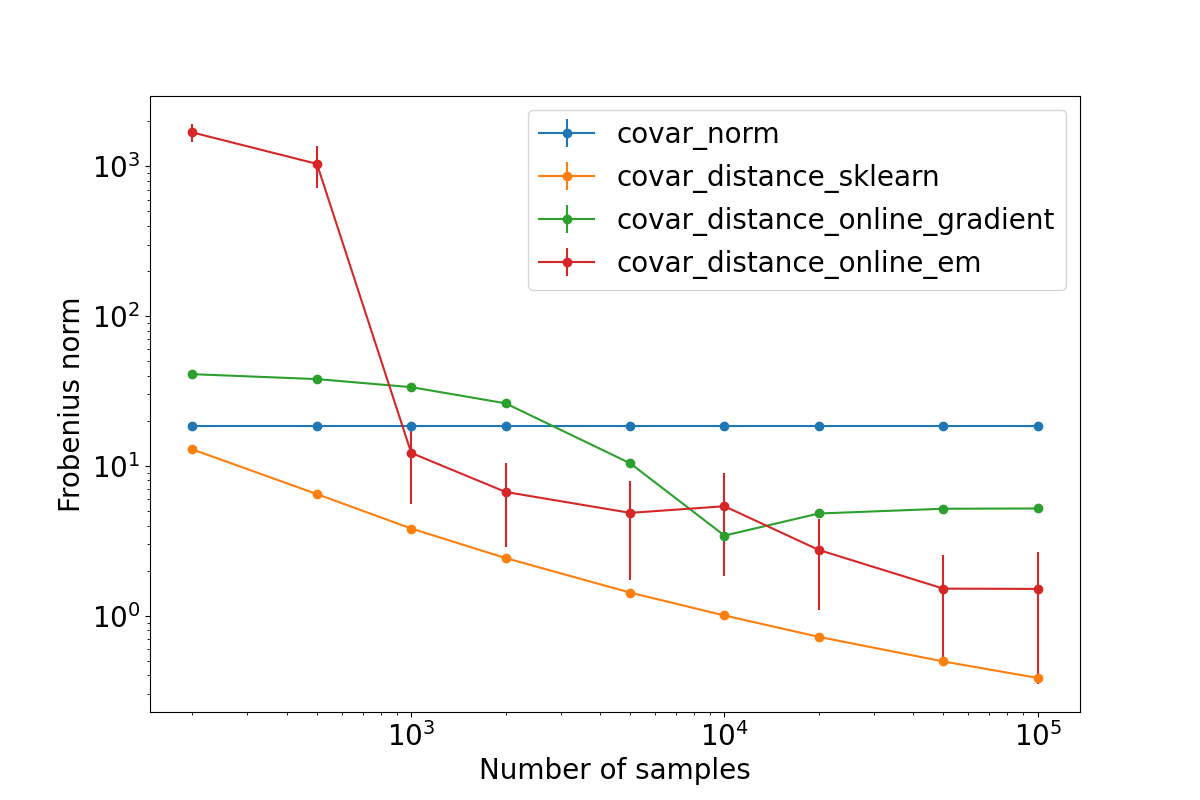
\includegraphics[width=70mm]{plots/online_fa_covar_distance__observation_dim=1000__latent_dim=10__spectrum_min=0__spectrum_max=1.png}
		 & 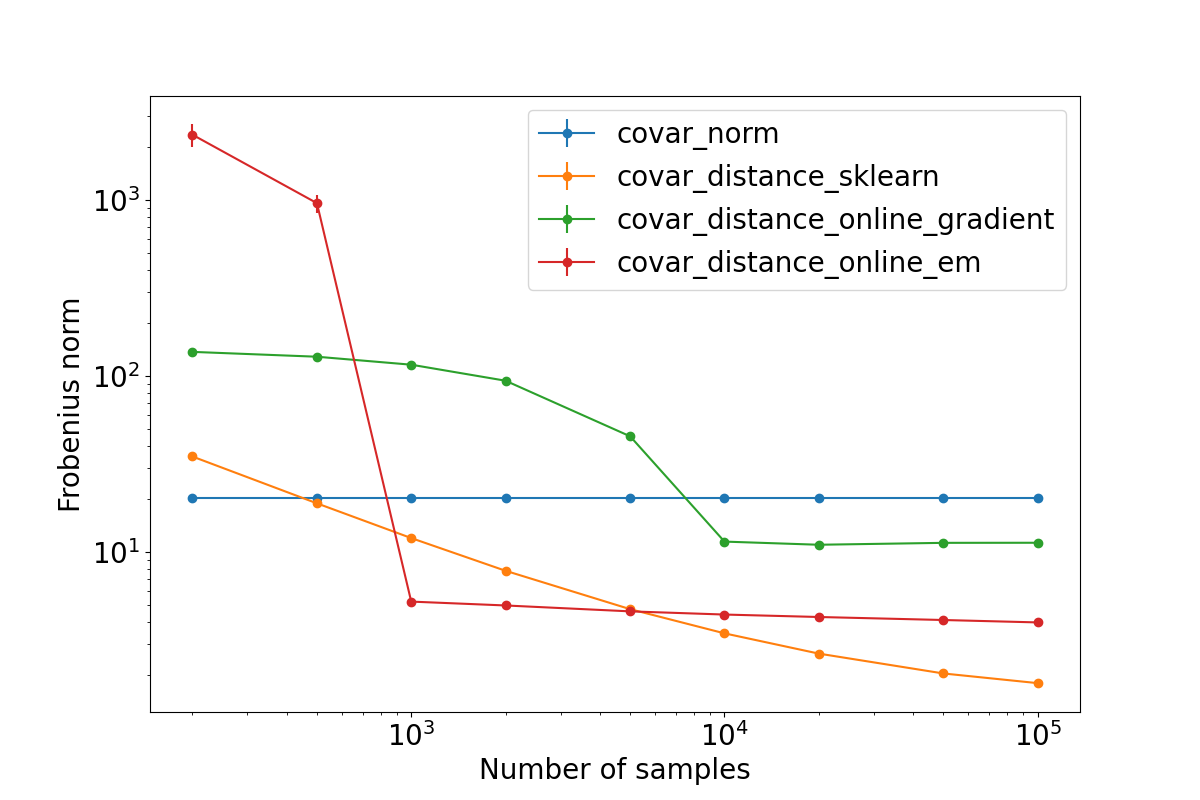
\includegraphics[width=70mm]{plots/online_fa_covar_distance__observation_dim=1000__latent_dim=100__spectrum_min=0__spectrum_max=1.png} \\
		 (a) $d=1000$, $K=10$, $s^2 \sim \mathcal{U}(0, 1)$ 
		 & (b) $d=1000$, $K=100$, $s^2 \sim \mathcal{U}(0, 1)$\\[6pt]
		 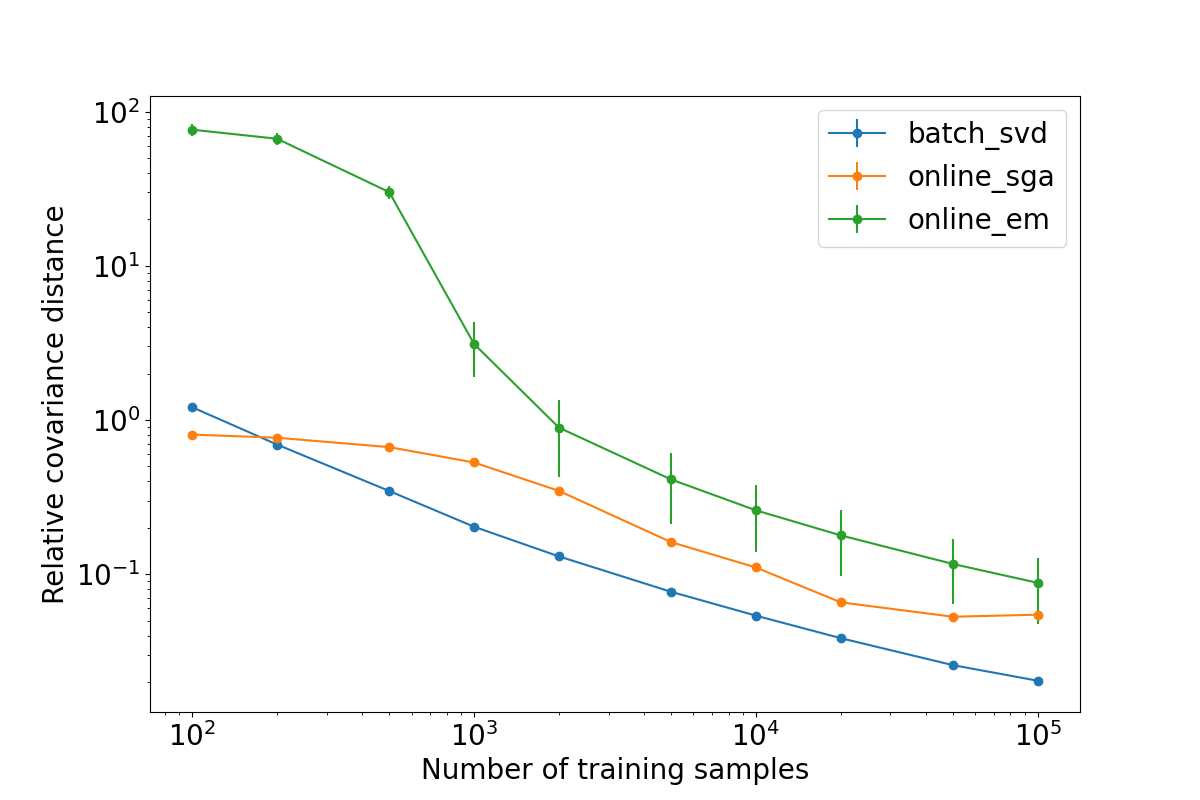
\includegraphics[width=70mm]{plots/online_fa_covar_distance__observation_dim=1000__latent_dim=10__spectrum_min=1__spectrum_max=10.png}
		 & 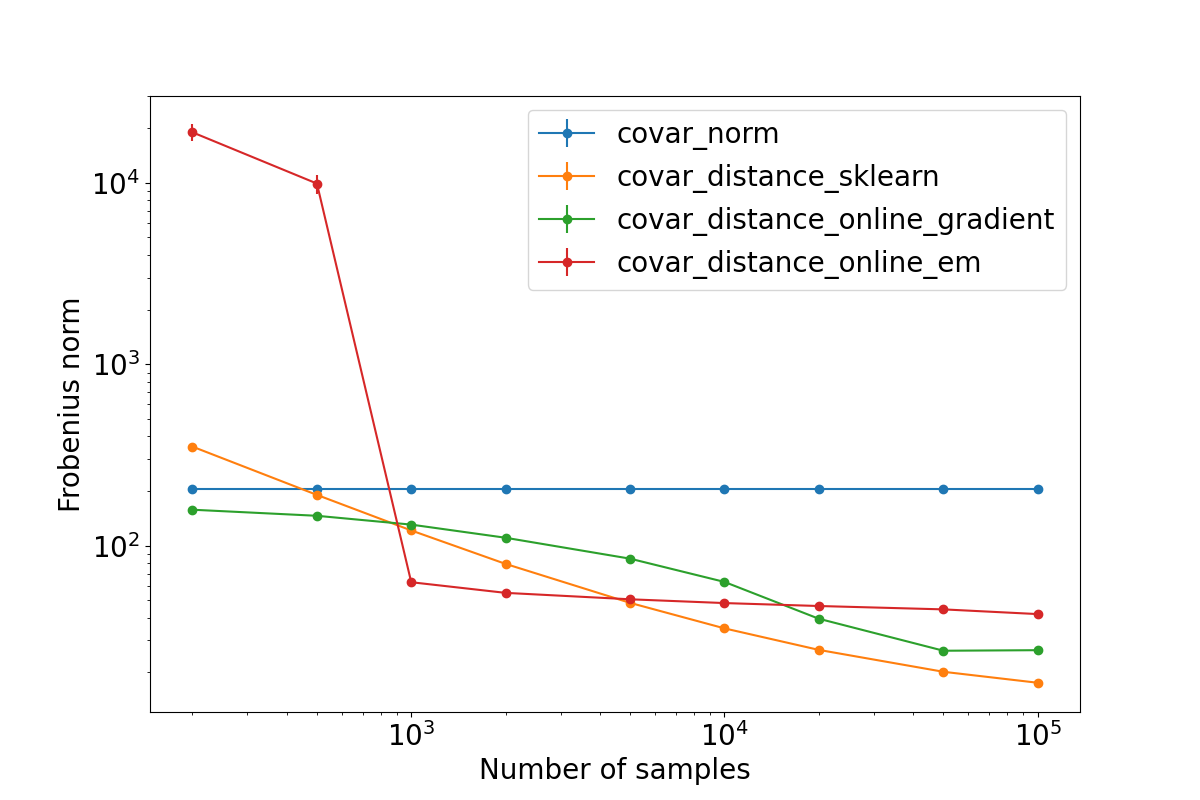
\includegraphics[width=70mm]{plots/online_fa_covar_distance__observation_dim=1000__latent_dim=100__spectrum_min=1__spectrum_max=10.png} \\
		 (c) $d=1000$, $K=10$, $s^2 \sim \mathcal{U}(1, 10)$ 
		 & (d) $d=1000$, $K=100$, $s^2 \sim \mathcal{U}(1, 10)$\\[6pt]
	\end{tabular}
	\caption{The distance of the estimated FA covariance matrices from the true covariance matrix as a function of the number of samples used to learn the models. The blue line shows the Frobenius norm of the true covariance matrix, while the orange, green and red lines shown the Frobenius norm of the difference between the true covariance matrix and the estimate covariance matrix for the scikit-learn batch algorithm, online gradient ascent and online EM, respectively. Each data point shows the mean value over ten trials with different random seeds, and standard error bars are also plotted. \textbf{(a)} The latent dimension of the FA model is equal to 10 and the spectrum, which controls the conditioning number of the true covariance matrix, is sampled from the uniform distribution with range $[0, 1]$. \textbf{(b)} The latent dimension is equal to 100 and the spectrum range is $[0, 1]$. \textbf{(c)} The latent dimension is equal to 10 and the spectrum range is $[1, 10]$. \textbf{(d)} The latent dimension is equal to 100 and the spectrum range is $[1, 10]$.}
	\label{fig:fa_covar_distance}
\end{figure}


\begin{figure}[!htbp] 
	\begin{tabular}{cc}
		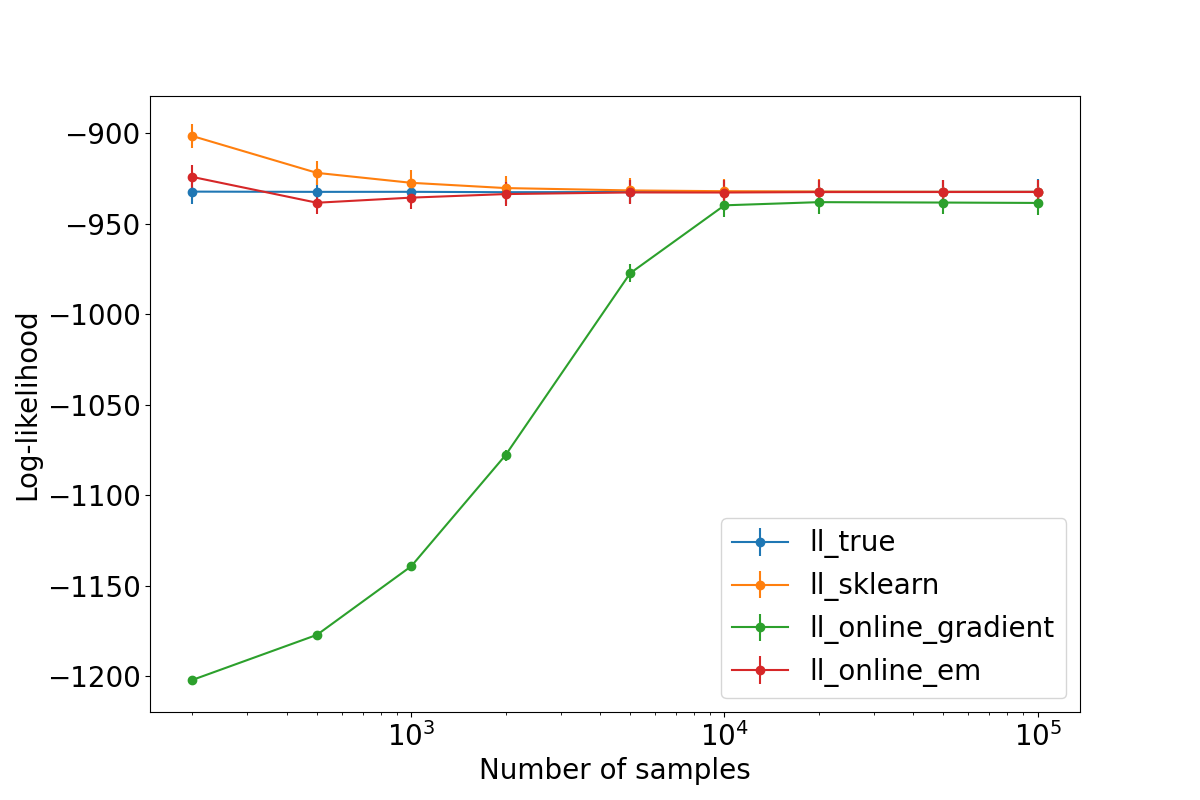
\includegraphics[width=70mm]{plots/online_fa_log_likelihood__observation_dim=1000__latent_dim=10__spectrum_min=0__spectrum_max=1.png}
		& 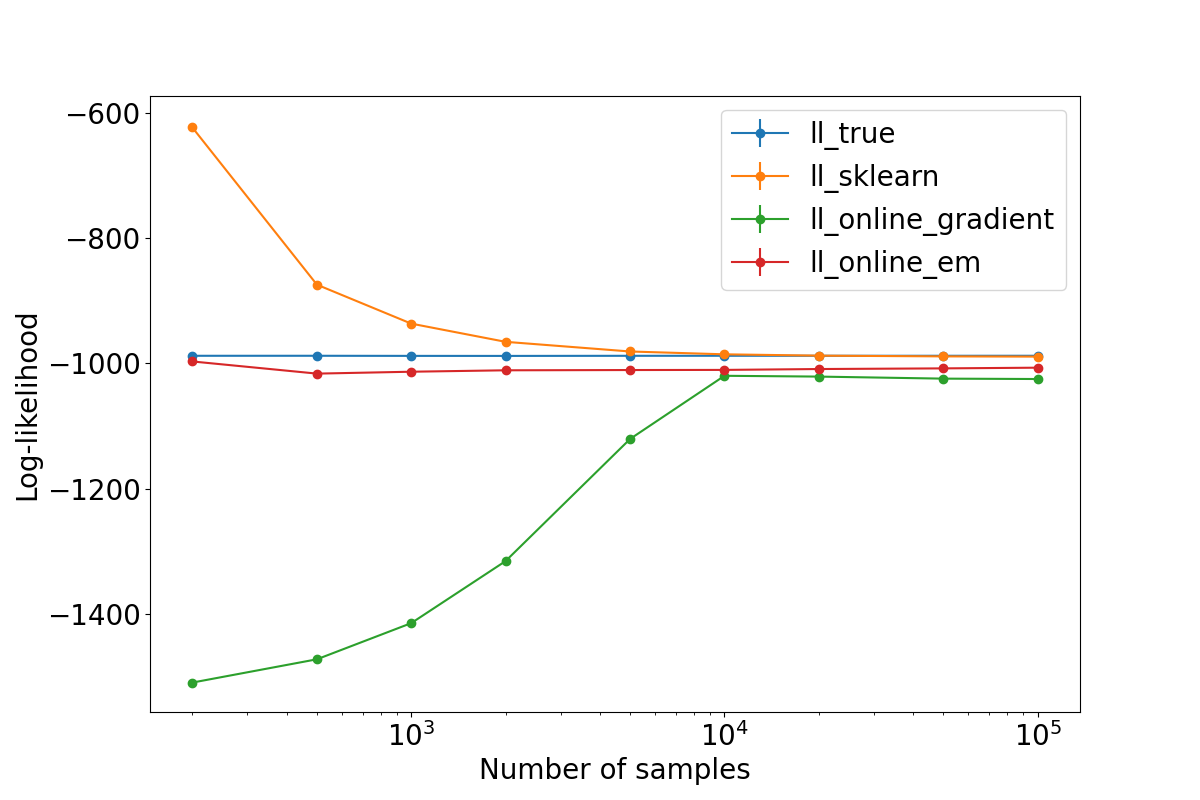
\includegraphics[width=70mm]{plots/online_fa_log_likelihood__observation_dim=1000__latent_dim=100__spectrum_min=0__spectrum_max=1.png} \\
		(a) $d=1000$, $K=10$, $s^2 \sim \mathcal{U}(0, 1)$ 
		 & (b) $d=1000$, $K=100$, $s^2 \sim \mathcal{U}(0, 1)$\\[6pt] 
		 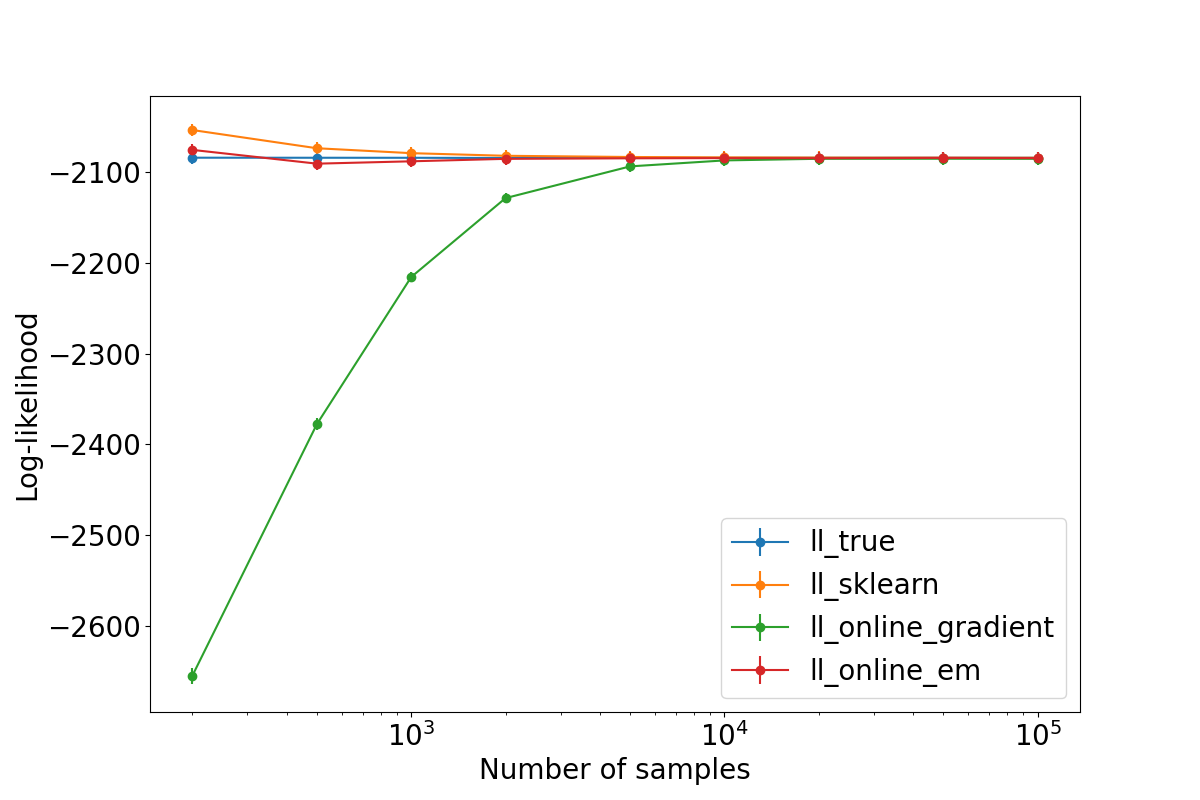
\includegraphics[width=70mm]{plots/online_fa_log_likelihood__observation_dim=1000__latent_dim=10__spectrum_min=1__spectrum_max=10.png} 
		 & 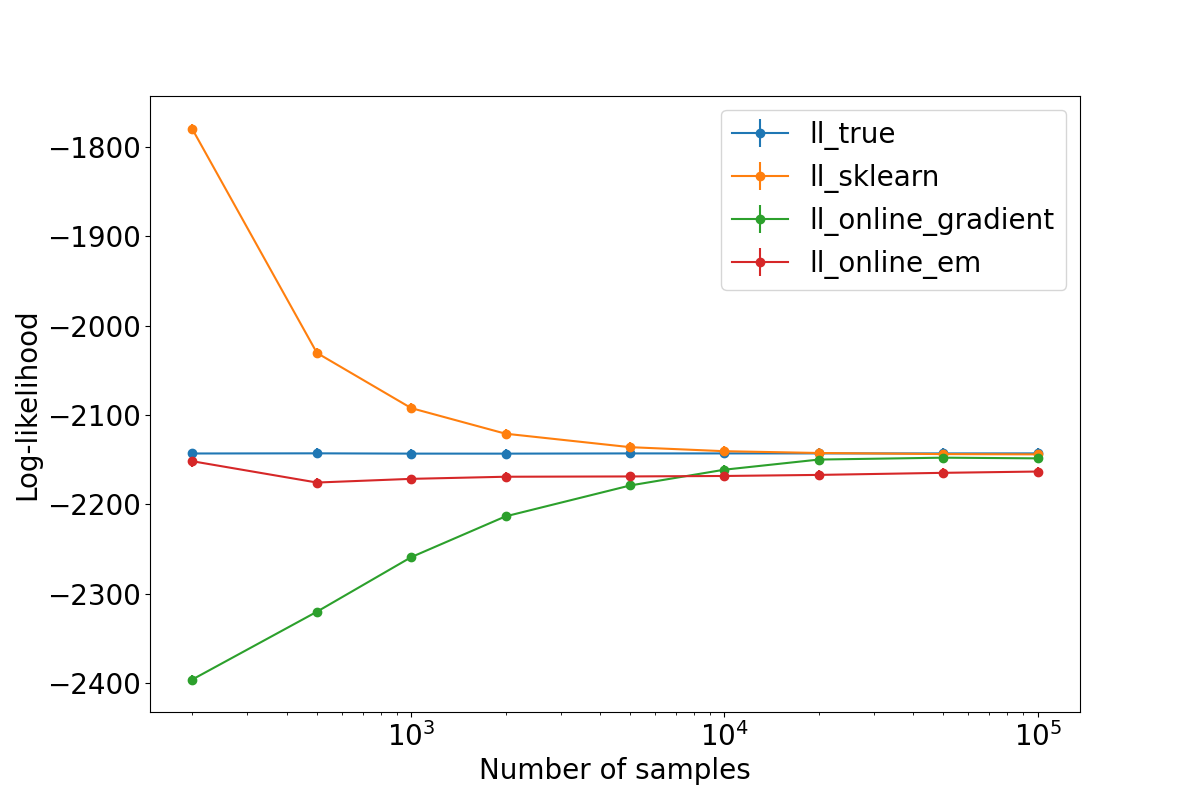
\includegraphics[width=70mm]{plots/online_fa_log_likelihood__observation_dim=1000__latent_dim=100__spectrum_min=1__spectrum_max=10.png} \\
		 (c) $d=1000$, $K=10$, $s^2 \sim \mathcal{U}(1, 10)$ 
		 & (d) $d=1000$, $K=100$, $s^2 \sim \mathcal{U}(1, 10)$\\[6pt]
	\end{tabular}
	\caption{The log-likelihood of the true and estimated FA models. The blue line shows the log-likelihood of the true FA model, while the orange, green and red lines shown the log-likelihood of the models estimated by the scikit-learn batch algorithm, online gradient ascent and online EM, respectively. Each data point shows the mean value over ten trials with different random seeds, and standard error bars are also plotted. \textbf{(a)} The latent dimension of the FA model is equal to 10 and the spectrum, which controls the conditioning number of the true covariance matrix, is sampled from the uniform distribution with range $[0, 1]$. \textbf{(b)} The latent dimension is equal to 100 and the spectrum range is $[0, 1]$. \textbf{(c)} The latent dimension is equal to 10 and the spectrum range is $[1, 10]$. \textbf{(d)} The latent dimension is equal to 100 and the spectrum range is $[1, 10]$.}
	\label{fig:fa_log_likelihood}
\end{figure}



\chapter{Conclusions}

%\section{Final Reminder}
%
%The body of your dissertation, before the references and any appendices,
%\emph{must} finish by page~40. The introduction, after preliminary material,
%should have started on page~1.
%
%You may not change the dissertation format (e.g., reduce the font
%size, change the margins, or reduce the line spacing from the default
%1.5 spacing). Over length or incorrectly-formatted dissertations will
%not be accepted and you would have to modify your dissertation and
%resubmit.  You cannot assume we will check your submission before the
%final deadline and if it requires resubmission after the deadline to
%conform to the page and style requirements you will be subject to the
%usual late penalties based on your final submission time.

\bibliographystyle{plain}
\bibliography{main}

%% You can include appendices like this:
% \appendix
%
% \chapter{First appendix}
%
% \section{First section}
%
% Markers do not have to consider appendices. Make sure that your contributions
% are made clear in the main body of the dissertation (within the page limit).

\end{document}